\documentclass[journal]{IEEEtran}
\usepackage{amsmath,amssymb,amsthm}
\usepackage{graphicx}
\usepackage{booktabs}
\usepackage{multirow}
\usepackage{url}
\usepackage[hidelinks]{hyperref}
\usepackage{cite}

\newtheorem{proposition}{Proposition}
\newtheorem{corollary}{Corollary}
\newcommand{\BA}{\mathrm{BA}}
\newcommand{\EEGNETPRE}{[pending X04]}

\begin{document}

\title{Per-Epoch Normalization Writes the Evoked Response Into the Pre-Stimulus Interval: An Exact Identity, an Averaging Law, and a Spiking-Reservoir Case Study}

\author{Andrew~A.~Lane,
        Wendy~Tang,
        and~Brady~D.~Nelson%
\thanks{A. A. Lane is with the Department of Mathematics and Computer Science, St. Joseph's University, Patchogue, NY 11772 USA (e-mail: andrew.a.lane@stonybrook.edu).}%
\thanks{W. Tang is with the Department of Electrical and Computer Engineering, Stony Brook University, Stony Brook, NY 11794 USA.}%
\thanks{B. D. Nelson is with the Department of Psychology, Stony Brook University, Stony Brook, NY 11794 USA.}}

\markboth{IEEE Transactions on Neural Systems and Rehabilitation Engineering}%
{Lane \MakeLowercase{\textit{et al.}}: Per-Epoch Normalization and Pre-Stimulus Leakage}

\maketitle

\begin{abstract}
Scaling each EEG epoch by its own mean and standard deviation is a common preprocessing step in decoding pipelines. We prove that for a baseline-corrected epoch this step maps the pre-stimulus mean onto a sign-flipped, rescaled copy of the post-stimulus mean, so any causal encoder receives post-stimulus information before the stimulus occurs. We derive an averaging law under which the discriminability of the leaked feature grows as the square root of the number of averaged trials, which predicts a small effect in single-trial decoding and a large effect in decoding of averaged, participant-level data. On 211 participants of an affective-picture ERP cohort, pre-stimulus channel means decode three affective conditions at 0.542 balanced accuracy under per-epoch z-scoring against 0.346 under pre-stimulus scaling (chance 0.333). A spiking reservoir from the ARSPI-Net framework, simulated only up to stimulus onset, decodes at 0.420, and the published operating point of that reservoir, 0.487, falls to 0.294 under leak-free scaling, a result reproduced by an independent implementation. EEGNet trained on pre-stimulus samples alone reaches \EEGNETPRE. On five paradigms of the public ERP CORE dataset, the across-participant leak reaches 0.573 to 0.715 in four paradigms and is weakest in the mismatch negativity, and the square-root law predicts the within-participant leak from single-trial accuracy alone. Three of ten widely used EEG decoding codebases scale each sample by its own statistics, and 70\% of 40 recent decoding papers do not report their scaling. Scaling with pre-stimulus or training statistics and reporting pre-stimulus decoding as a null check remove the leak.
\end{abstract}

\begin{IEEEkeywords}
EEG decoding, event-related potentials, normalization, data leakage, spiking reservoir, ARSPI-Net, evaluation methodology.
\end{IEEEkeywords}

\section{Introduction}
\IEEEPARstart{E}{vent-related} potentials (ERPs) are time-locked measurements of evoked neural dynamics, and decoding them with machine learning has become a standard engineering route to brain-computer interfaces, clinical markers, and affective state estimation \cite{blankertz2011erp,roy2019review,craik2019review}. Every decoding pipeline places a scaling step between the recorded epoch and the model. A widespread choice scales each epoch and channel by its own statistics, subtracting the epoch mean and dividing by the epoch standard deviation. The step is motivated by numerical conditioning and by the large between-recording differences in EEG amplitude, and a recent normalization benchmark reports that window-level, within-channel normalization gives the highest supervised performance among the strategies it compared \cite{truong2025normalization}.

Preprocessing choices shape what a decoder measures. High-pass filtering displaces multivariate patterns into activity-silent periods \cite{vandriel2021highpass} and creates artifactual ERP effects of opposite polarity before a true effect \cite{tanner2015highpass}. A multiverse analysis of the ERP CORE dataset reports significant decoding clusters that extend into the baseline period for some forking paths \cite{kessler2025preprocessing}. Benchmarking studies in this journal show that EEG results are sensitive to preprocessing \cite{robbins2020sensitive} and that preprocessing depth changes deep-learning performance across six tasks \cite{delpup2025more}. Leakage through data partitioning is now widely documented \cite{brookshire2024leakage,kapoor2023leakage}. Normalization that uses each epoch's own statistics is a different kind of leakage. It moves information along the time axis inside a single observation, so subject-grouped partitioning and train-only scaling leave it untouched. Its closest precedent is the detrending analysis of \cite{vandriel2021highpass}, which showed empirically that a polynomial fitted to a whole trial displaces decodable information into the baseline and that masking the response during the fit prevents it. Subtracting an epoch mean is the zero-order case of such a fit. Three things remain open after that work, and they are the subject of this one: a closed form for what the normalization step writes into the pre-stimulus interval, the role of the dividing statistic, which no masking of a subtracted trend addresses, and a law for how large the effect is in a given decoding regime. The step also now sits by default in deep-learning toolchains. A recent foundation-model benchmark compares z-scoring, unit rescaling, and division by each trial's 95th amplitude percentile as its normalization choices \cite{wu2025adabrain}, whereas causal alternatives such as exponential moving standardization \cite{schirrmeister2017deep} were designed for online use.

This work isolates that mechanism and quantifies it. It grows out of the temporal encoding stage of ARSPI-Net \cite{lane2023arspinet,lane2024arspinet,lane2026dissertation}, a fixed leaky integrate-and-fire (LIF) reservoir \cite{maass2002lsm} whose perturbation properties on affective ERPs were characterized at IEEE BIBM 2026 \cite{lane2026bibm}. The spike-count window of that reservoir lies mostly before stimulus onset, and its input epochs were z-scored over their full length. A fixed recurrent system read out before the stimulus provides an unusually clean probe. Any condition information in its state at onset can only enter through the scaling step.

The paper makes four contributions. First, it proves two exact identities. Through the subtracted statistic, per-epoch z-scoring maps the pre-stimulus mean of a baseline-corrected epoch onto a sign-flipped, rescaled copy of the post-stimulus mean. Through the dividing statistic, it writes post-stimulus energy into every pre-stimulus variance, including under scale-only normalization. A causal encoder therefore receives post-stimulus information before the stimulus (Sec.~\ref{sec:theory}). Second, it derives an averaging law that predicts the size of the effect from single-trial statistics. Discriminability of the leaked feature grows as the square root of the number of averaged trials, which places trial-averaged, participant-level decoding (the regime of many clinical and individual-differences studies) in the high-leakage regime and single-trial decoding in the low-leakage regime. Third, it tests these predictions on 211 participants of an affective-picture ERP cohort and on five paradigms of the public ERP CORE dataset \cite{kappenman2021erpcore}, with linear readouts, the ARSPI-Net reservoir, and a trained EEGNet \cite{lawhern2018eegnet}. Fourth, it re-evaluates the BIBM 2026 reservoir result under scaling that uses no post-stimulus sample and gives a reporting rule with a pre-stimulus null test that any pipeline can run.

\section{Theory}\label{sec:theory}

\subsection{Observation Model}
Consider one channel of one epoch, $x(t)$ for $t=1,\dots,T$, with pre-stimulus index set $\mathcal{P}$ of size $T_0$ and post-stimulus set $\mathcal{Q}$ of size $T_1=T-T_0$. Write $x(t)=s_y(t)+n(t)$, where $s_y$ is the evoked response for condition $y$, zero on $\mathcal{P}$, and $n$ is zero-mean background activity. Baseline correction subtracts the pre-stimulus mean, so that
\begin{equation}
\textstyle\sum_{t\in\mathcal{P}} x(t)=0. \label{eq:bc}
\end{equation}
Denote the post-stimulus mean by $\bar{x}_\mathcal{Q}=T_1^{-1}\sum_{t\in\mathcal{Q}}x(t)$. The following scalings are compared. Per-epoch z-scoring uses the epoch mean $m=T^{-1}\sum_t x(t)$ and standard deviation $\hat\sigma$,
\begin{equation}
z(t)=\frac{x(t)-m}{\hat\sigma}. \label{eq:z}
\end{equation}
A post-stimulus variant replaces $(m,\hat\sigma)$ by the mean and standard deviation over $\mathcal{Q}$. Epoch centering $x(t)-m$ and scale-only normalization $x(t)/\hat\sigma$ apply each half of \eqref{eq:z} alone. Pre-stimulus scaling divides by the standard deviation over $\mathcal{P}$, $\tilde{x}(t)=x(t)/\hat\sigma_\mathcal{P}$, and the unscaled signal is kept in microvolts.

\subsection{The Leakage Identity}
\begin{proposition}[Location route]\label{prop:identity}
For any epoch, with $\bar{x}_\mathcal{P}$ and $\bar{x}_\mathcal{Q}$ the pre- and post-stimulus means,
\begin{equation}
\bar{z}_\mathcal{P}=\frac{T_1}{T}\,\frac{\bar{x}_\mathcal{P}-\bar{x}_\mathcal{Q}}{\hat\sigma}. \label{eq:general}
\end{equation}
For a baseline-corrected epoch, $m=(T_1/T)\,\bar{x}_\mathcal{Q}$, and for every $t\in\mathcal{P}$
\begin{equation}
z(t)=\frac{x(t)}{\hat\sigma}-\frac{T_1}{T}\,\frac{\bar{x}_\mathcal{Q}}{\hat\sigma},
\qquad
\bar{z}_\mathcal{P}=-\frac{T_1}{T}\,\frac{\bar{x}_\mathcal{Q}}{\hat\sigma}. \label{eq:identity}
\end{equation}
Under the post-stimulus variant, $\bar{z}_\mathcal{P}=-\bar{x}_\mathcal{Q}/\hat\sigma_\mathcal{Q}$.
\end{proposition}
\begin{proof}
Write $m=(T_0\bar{x}_\mathcal{P}+T_1\bar{x}_\mathcal{Q})/T$, so $\bar{x}_\mathcal{P}-m=(T_1/T)(\bar{x}_\mathcal{P}-\bar{x}_\mathcal{Q})$, which gives \eqref{eq:general}. Setting $\bar{x}_\mathcal{P}=0$ by \eqref{eq:bc} gives \eqref{eq:identity}. The variant follows in the same way.
\end{proof}

Both forms are exact, and \eqref{eq:general} needs no assumption about baseline correction. After baseline correction the pre-stimulus mean of a z-scored epoch carries no pre-stimulus information: it is the post-stimulus mean amplitude, sign-flipped and scaled by $T_1/(T\hat\sigma)$. A sustained, one-signed condition difference, such as the late positive potential \cite{hajcak2010lpp} or the P3, therefore appears at every pre-stimulus sample at once.

\begin{proposition}[Scale route]\label{prop:scale}
For a baseline-corrected epoch with interval variances $s_\mathcal{P}^2$ and $s_\mathcal{Q}^2$,
\begin{equation}
\hat\sigma^2=\frac{T_0}{T}\,s_\mathcal{P}^2+\frac{T_1}{T}\,s_\mathcal{Q}^2+\frac{T_0T_1}{T^2}\,\bar{x}_\mathcal{Q}^2. \label{eq:scale}
\end{equation}
Under scale-only normalization $x(t)/\hat\sigma$, the pre-stimulus mean is zero and the pre-stimulus variance is $s_\mathcal{P}^2/\hat\sigma^2$.
\end{proposition}
\begin{proof}
$\hat\sigma^2=T^{-1}\sum_t x(t)^2-m^2$. By \eqref{eq:bc}, $\sum_\mathcal{P}x^2=T_0s_\mathcal{P}^2$ and $\sum_\mathcal{Q}x^2=T_1(s_\mathcal{Q}^2+\bar{x}_\mathcal{Q}^2)$. Substituting $m=(T_1/T)\bar{x}_\mathcal{Q}$ gives \eqref{eq:scale}.
\end{proof}

The denominator contains the energy of the evoked response. Dividing by it leaves first-order pre-stimulus features untouched and writes post-stimulus energy into every second-order feature and any nonlinear encoder. The propositions make separate predictions: a whole-epoch location statistic (mean, minimum) leaks into pre-stimulus means, and a whole-epoch scale statistic (standard deviation, range, amplitude percentile) leaks into pre-stimulus variances.

\begin{corollary}[Causal encoders]\label{cor:causal}
Let $\xi_t=\Phi(\xi_{t-1},u_t)$ be any causal state-space encoder and let $\xi_{T_0}$ be its state at stimulus onset. Driven by $u=z$, $\xi_{T_0}$ is a function of $(x_\mathcal{P},\bar{x}_\mathcal{Q},\hat\sigma)$ and can carry information about $y$ even when $I(y;x_\mathcal{P})=0$. The same holds for $u=x/\hat\sigma$ through \eqref{eq:scale}. Driven by pre-stimulus scaling, $\xi_{T_0}$ is a function of $x_\mathcal{P}$ alone, and the data processing inequality gives $I(y;\xi_{T_0})\le I(y;x_\mathcal{P})$.
\end{corollary}

The corollary gives a falsifiable test for any temporal model: restricted to pre-stimulus samples, it decodes at chance under scaling that never touches $\mathcal{Q}$.

\subsection{The Averaging Law}
Let trial $i$ of condition $y$ have post-stimulus mean pattern $\bar{\mathbf{x}}^{(i)}_\mathcal{Q}=\boldsymbol\mu_y+\mathbf{e}_i$ across channels, with $\mathbf{e}_i$ independent with covariance $\Sigma_e$. An average of $k$ trials has the same condition means and covariance $\Sigma_e/k$. Treating $\hat\sigma$ as approximately constant, which holds when it is estimated from many samples, the leaked pattern \eqref{eq:identity} is an affine image of the post-stimulus mean, and its Mahalanobis separation is
\begin{equation}
D(k)=\sqrt{k}\,D(1),\qquad D(1)^2=\Delta\boldsymbol\mu^\top\Sigma_e^{-1}\Delta\boldsymbol\mu. \label{eq:law}
\end{equation}
For two equal-covariance Gaussian classes the optimal balanced accuracy is $\Phi(D/2)$, which yields the parameter-free prediction
\begin{equation}
\BA(k)=\Phi\!\left(\sqrt{k}\;\Phi^{-1}\!\big(\BA(1)\big)\right). \label{eq:pred}
\end{equation}
Equation \eqref{eq:law} is exact under its model: independent trials, a common covariance, and a fixed $\hat\sigma$. Equation \eqref{eq:pred} adds Gaussian classes and an optimal linear readout, so for a decoder estimated from a finite sample it is an approximation, tested in Sec.~\ref{sec:results}. Single-trial decoding sits at $k=1$, where the leak is small. Participant-level decoding of averaged ERPs sits at $k$ equal to the number of retained trials. Across participants the covariance becomes $\Sigma_b+\Sigma_e/k$, so participant variability bounds the leak.

\section{Materials and Methods}\label{sec:methods}

\subsection{Datasets}
\emph{SHAPE.} Trial-averaged affective ERPs from the Stress, Health, and the Psychophysiology of Emotion project \cite{shape}, recorded during passive viewing of negative, neutral, and pleasant pictures. After exclusion of one participant with a recording anomaly, 211 participants contributed three condition averages each (633 observations, chance $1/3$). Each epoch had 34 scalp channels at 1024~Hz and was baseline-corrected over the 200~ms before onset. As in \cite{lane2026bibm}, every fourth of the first 1024 samples was analysed, giving 256 samples at 256~Hz from $-200$ to $+800$~ms with onset at sample 51. The analysed pre-stimulus window was a subsample of the baseline window, so \eqref{eq:bc} held approximately in this cohort.

\emph{ERP CORE.} Five stimulus-locked paradigms of the public ERP CORE resource \cite{kappenman2021erpcore}, each with 40 participants: N170 (faces versus cars), P3 (rare versus frequent targets), N400 (unrelated versus related word pairs), N2pc (left versus right target), and MMN (deviants versus standards). The delivered epochs were ICA-corrected, baseline-corrected over $-200$ to $0$~ms, sampled at 256~Hz, and spanned $-200$ to $+797$~ms. Trials flagged by the provided artifact detection were removed and the 28 scalp channels were kept. The response-locked ERN and LRP paradigms were excluded, since motor preparation makes their pre-event interval non-null.

\subsection{Scalings}
Each epoch and channel was scaled by one of the rules of Sec.~\ref{sec:theory}: per-epoch z-scoring (\texttt{epoch\_z}), z-scoring with post-stimulus statistics (\texttt{post\_z}), division by the pre-stimulus standard deviation (\texttt{pre\_sd}), and no scaling (\texttt{none}). On SHAPE a fifth rule divided each channel by one cohort-wide standard deviation (\texttt{global\_sd}). Four further rules separated the routes of Propositions~\ref{prop:identity} and~\ref{prop:scale} and reproduced the transforms of the codebase audit: epoch centering $x-m$, scale-only normalization $x/\hat\sigma$, division by the 95th percentile of $|x|$ over the epoch (the BIOT form \cite{yang2023biot}), and per-epoch min-max scaling into $[-1,1]$ (the DN3 form used by BENDR \cite{kostas2021bendr}).

\subsection{Encoders}
The \emph{pre-stimulus mean} encoder averaged each channel over the pre-stimulus window ($-164$ to $0$~ms on SHAPE, $-200$ to $0$~ms on ERP CORE), and a six-bin version kept the temporal profile. The \emph{pre-stimulus log-SD} encoder took the logarithm of each channel's standard deviation over the same window, a second-order feature that is blind to any offset. The \emph{ERP-window} encoder was the BIBM baseline, with three window means per channel \cite{lane2026bibm}.

The \emph{ARSPI-Net reservoir} \cite{lane2026bibm} had 256 LIF neurons driven independently by each channel, with membrane update $\mathbf{v}_t=(1-\beta)(1-\mathbf{z}_{t-1})\odot\mathbf{v}_{t-1}+W\mathbf{z}_{t-1}+W_\mathrm{in}u_t$, spikes $\mathbf{z}_t=\mathbb{1}[\mathbf{v}_t\ge\vartheta]$, threshold subtraction and rectification, $\beta=0.05$, $\vartheta=0.5$, Xavier-uniform weights (seed 42), and spectral radius $\rho=0.9$. Spike counts in six equal bins were compressed by one 64-component PCA basis shared across channels and fitted on training participants only. The BIBM read-out window spanned samples 10 to 69 ($-160$ to $+73$~ms). The \emph{onset-truncated} reservoir stopped its simulation at stimulus onset and read samples 9 to 50, so it never received a post-stimulus sample.

\emph{EEGNet-8,2} \cite{lawhern2018eegnet} was trained with the recipe of \cite{lane2026bibm} (80 epochs, train-only per-channel standardization) on the full epoch and, separately, on the pre-stimulus samples alone, with a 32-sample temporal kernel for the shorter input.

\subsection{Evaluation}
On SHAPE the BIBM protocol was kept exactly: \texttt{StratifiedGroupKFold} with five folds and seeds 42 to 46, participants as groups, train-only standardization, and a class-balanced L2 logistic readout ($C=1$). Out-of-fold class probabilities were summed over the five partitions, and 95\% intervals came from 4000 bootstrap resamples of participants, each kept with its three observations. Contrasts were paired differences under the same resampling, and nulls permuted labels within participants.

On ERP CORE the test statistic was registered in the public dissertation repository \cite{repo_disso} before any ERP CORE result was computed: the 28-channel pattern of each 15.6~ms bin was decoded separately, and accuracy was averaged over the bins centered in $[-200,0)$~ms. In the \emph{across-participant} regime trials were scaled, then averaged per participant and condition, giving 80 observations per paradigm, and each bin was decoded with participant-grouped five-fold cross-validation repeated five times, standardization, and an L2 logistic readout. Significance came from 200 permutations that swapped each participant's two labels with probability one half, which preserves the paired structure of the design. For per-epoch z-scoring and unscaled input the test was repeated with 2000 and 500 permutations, and $p$ values were Holm-adjusted over the five paradigms. In the \emph{within-participant} regime single trials were decoded per bin with shrinkage linear discriminant analysis under stratified five-fold cross-validation repeated twice, and participant means were tested against 0.5 with a one-sample $t$-test.

\subsection{Averaging-Law Experiment}
To test \eqref{eq:pred}, trials of each ERP CORE participant were first split into five stratified folds. Within each fold, 40 pseudo-trials per class were formed separately from the training and test pools by averaging $k\in\{1,2,4,8,16\}$ distinct trials. Pseudo-trials were scaled and decoded with the same per-bin statistic and shrinkage LDA. The predictions for the ERP CORE, averaging-law, EEGNet, and route experiments were committed to the public code repository \cite{repo_sequel} before those experiments were run.

\section{Results}\label{sec:results}
\subsection{The Identity on Real Data}
On SHAPE, the pre-stimulus mean of each z-scored epoch and channel correlates at $r=0.9965$ with $-m/\hat\sigma$ computed from the unscaled epoch (Fig.~\ref{fig:mechanism}c), as Proposition~\ref{prop:identity} predicts for a pre-stimulus window that approximates the baseline window. The two feature sets decode at BA 0.542 and 0.543 under the BIBM protocol, and their out-of-fold predictions agree on 95.9\% of observations. In microvolts the three conditions overlap before onset, and after z-scoring the neutral condition sits about 0.3 standard deviations above the two emotional conditions throughout the pre-stimulus interval (Fig.~\ref{fig:mechanism}a,b). This offset is the late positive potential of the emotional conditions \cite{hajcak2010lpp}, sign-flipped and moved to $t<0$.

\begin{figure*}[t]
\centering
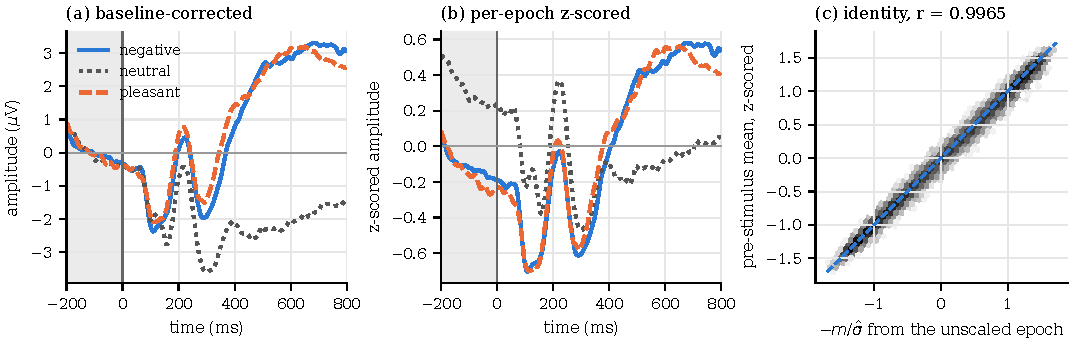
\includegraphics[width=\textwidth]{figures/fig_mechanism.pdf}
\caption{The leakage identity on SHAPE (211 participants, grand averages over participants and 34 channels). (a) Baseline-corrected ERPs overlap before onset (gray). (b) After per-epoch z-scoring the pre-stimulus interval is offset by condition. (c) Pre-stimulus mean of each z-scored epoch and channel against $-m/\hat\sigma$ of the unscaled epoch, log-density, $r=0.9965$ (dashed: identity line).}
\label{fig:mechanism}
\end{figure*}

\subsection{Pre-Stimulus Decoding on SHAPE}
Table~\ref{tab:shape} reports every encoder under every scaling. Under per-epoch z-scoring the 34 pre-stimulus channel means decode the three affective conditions at BA 0.542 [0.507, 0.575], against a within-participant permutation null with 95th percentile 0.371 and maximum 0.393 over 200 permutations. Under pre-stimulus scaling the same feature scores 0.346 [0.313, 0.381], inside its null (95th percentile 0.370). The paired difference between the two scalings is $+0.196$ [$+0.148$, $+0.242$] BA.

Time-resolved decoding locates the effect in time (Fig.~\ref{fig:shape}a). Under per-epoch z-scoring the first bin whose interval excludes chance is centered at $-193$~ms, the first bin of the epoch, and the mean pre-stimulus BA is 0.511. Under pre-stimulus scaling and under unscaled input the first such bin is centered at $+88$~ms, and the pre-stimulus means are 0.325 and 0.319. Z-scoring also attenuates the late structure that carries the genuine condition information: mean BA over 400 to 800~ms is 0.543 under z-scoring against 0.594 unscaled, with peaks of 0.602 and 0.632.

\begin{figure*}[t]
\centering
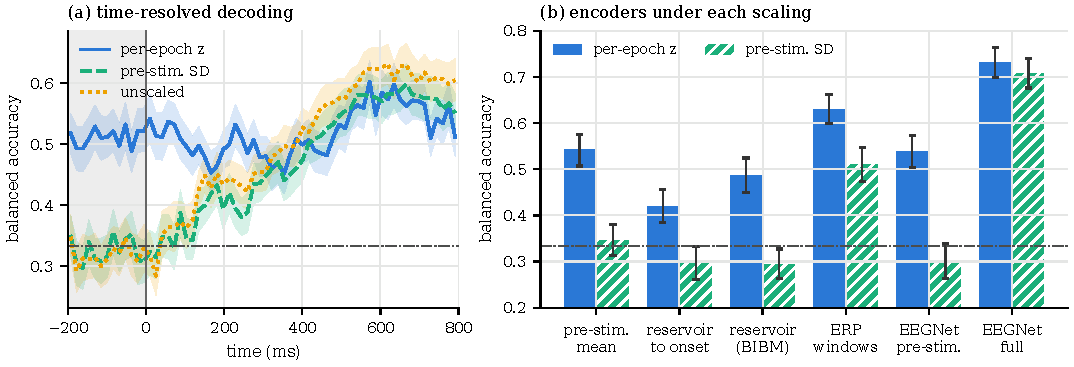
\includegraphics[width=\textwidth]{figures/fig_shape.pdf}
\caption{SHAPE, three affective conditions, chance $1/3$ (dash-dot). (a) Time-resolved decoding of the 34-channel pattern in 15.6~ms bins with participant-bootstrap 95\% intervals. Under per-epoch z-scoring decoding is above chance from the first pre-stimulus bin. (b) Balanced accuracy of each encoder under each scaling with participant-bootstrap 95\% intervals. The onset-truncated reservoir never receives a post-stimulus sample.}
\label{fig:shape}
\end{figure*}

\subsection{The ARSPI-Net Reservoir}
Under per-epoch z-scoring the BIBM reservoir configuration reproduces the published operating point exactly, BA 0.487 [0.450, 0.524] against the reported 0.487 [0.447, 0.523] \cite{lane2026bibm}, at a firing rate of 0.124. Under pre-stimulus scaling the same reservoir scores 0.294 [0.262, 0.327], and unscaled it scores 0.316 [0.278, 0.354]. The paired difference attributable to scaling is $+0.192$ [$+0.142$, $+0.243$] BA, which accounts for the full margin of the BIBM result above chance. The firing rate changes little between these scalings (0.124 to 0.144), so the difference does not come from a change in operating regime.

The onset-truncated reservoir isolates Corollary~\ref{cor:causal}. Its simulation stops at stimulus onset, so its spike counts are a function of pre-stimulus input alone. Driven by z-scored epochs it decodes at 0.420 [0.384, 0.457], and driven by pre-stimulus-scaled epochs at 0.297 [0.261, 0.333]. A causal dynamical system that has not yet received the stimulus therefore classifies the affective response to it, and the information enters through $m$ and $\hat\sigma$.

The ERP-window baseline of BIBM is affected as well, because its first window spans the pre-stimulus baseline. It scores 0.630 [0.599, 0.662] under z-scoring and 0.545 [0.512, 0.578] unscaled, a paired difference of $+0.085$ [$+0.049$, $+0.122$].

\begin{table*}[t]
\centering
\caption{SHAPE: balanced accuracy (participant-bootstrap 95\% CI) by encoder and scaling. Three classes, chance 0.333; 211 participants, 633 observations. Only \texttt{epoch\_z} and \texttt{post\_z} use post-stimulus samples to scale earlier ones. A dash marks a combination not run.}
\label{tab:shape}
\begin{tabular}{lcccc}
\toprule
Encoder & \texttt{epoch\_z} & \texttt{post\_z} & \texttt{pre\_sd} & \texttt{none} \\
\midrule
Pre-stimulus mean (34) & 0.542 [0.507, 0.575] & 0.555 [0.518, 0.591] & 0.346 [0.313, 0.381] & 0.340 [0.303, 0.378] \\
Pre-stimulus, 6 bins (204) & 0.496 [0.460, 0.532] & 0.510 [0.474, 0.547] & 0.335 [0.303, 0.370] & 0.311 [0.276, 0.349] \\
Reservoir, truncated at onset & 0.420 [0.384, 0.457] & 0.498 [0.460, 0.536] & 0.297 [0.261, 0.333] & 0.292 [0.258, 0.330] \\
Reservoir, BIBM window & 0.487 [0.450, 0.524] & 0.464 [0.427, 0.504] & 0.294 [0.262, 0.327] & 0.316 [0.278, 0.354] \\
ERP windows (102) & 0.630 [0.599, 0.662] & 0.632 [0.596, 0.667] & 0.510 [0.474, 0.547] & 0.545 [0.512, 0.578] \\
EEGNet, pre-stimulus input & 0.539 [0.504, 0.573] & -- & 0.300 [0.264, 0.338] & -- \\
EEGNet, full epoch & 0.731 [0.700, 0.763] & -- & 0.708 [0.676, 0.739] & -- \\
\bottomrule
\end{tabular}
\end{table*}

\subsection{A Trained Network Learns the Leak}
EEGNet-8,2 trained on the pre-stimulus samples alone decodes the three affective conditions at 0.539 [0.504, 0.573] under per-epoch z-scoring and at 0.300 [0.264, 0.338] under pre-stimulus scaling, a paired difference of $+0.239$ [$+0.191$, $+0.288$]. Gradient training therefore finds the leaked offset unaided. On the full epoch the same network scores 0.731 [0.700, 0.763] under z-scoring, reproducing the BIBM value \cite{lane2026bibm}, and 0.708 [0.676, 0.739] under pre-stimulus scaling, a difference of $+0.023$ [$-0.005$, $+0.052$]. When the post-stimulus response is in view, the leak duplicates information the network already reads. Per-epoch scaling therefore matters for windows that include pre-stimulus samples and for latency claims.

\subsection{Replication on ERP CORE}
Table~\ref{tab:erpcore} and Fig.~\ref{fig:erpcore} report the pre-stimulus statistic for the five ERP CORE paradigms. Under both scalings that use no post-stimulus sample, every paradigm sits inside its permutation null in both regimes. Under per-epoch z-scoring, the across-participant statistic exceeds its null in the paradigms with a sustained one-signed condition difference: N170 at 0.573 ($p=0.0040$), P3 at 0.695 ($p=0.0005$), and N400 at 0.715 ($p=0.0005$) with 2000 permutations, or 0.008, 0.0025, and 0.0025 after Holm adjustment over the five paradigms. The post-stimulus variant gives 0.582, 0.703, and 0.724. The lateralized N2pc, whose condition difference reverses sign across hemispheres, also leaks across participants (0.597, $p=0.005$), because each channel's epoch mean carries its own signed contrast and the decoder reads the pattern across channels. One N2pc participant has no retained trial in one condition and is excluded from that paradigm.


Within participants, on single trials, the mechanism is present at the smaller magnitude the averaging law predicts for $k=1$. Under per-epoch z-scoring the N400 statistic is 0.537 ($t$-test $p=5.2\times10^{-8}$, 36 of 40 participants above 0.5), while N170 and P3 give 0.515 ($p=0.084$) and 0.504 ($p=0.052$). The post-stimulus variant reaches significance in all three (N170 0.520, $p=0.024$, P3 0.507, $p=0.018$, and N400 0.544, $p=1.3\times10^{-8}$).

Scaling the participant average directly, the order of the SHAPE pipeline, yields the same pattern (N170 0.569, P3 0.595, N400 0.717, each $p\le0.01$), and a decoder fed $-m/\hat\sigma$ of each average reaches 0.603, 0.630, and 0.790.

\begin{table*}[t]
\centering
\caption{ERP CORE: mean pre-stimulus decoding accuracy ($-200$ to $0$~ms, 15.6~ms bins), two classes, chance 0.5, 40 participants per paradigm. Across participants: trials scaled, then averaged; $p$ from 200 label permutations. Within participants: single trials; mean [95\% CI] and one-sample $t$-test $p$ against 0.5.}
\label{tab:erpcore}
\begin{tabular}{llcccc}
\toprule
Paradigm & Regime & \texttt{none} & \texttt{pre\_sd} & \texttt{epoch\_z} & \texttt{post\_z} \\
\midrule
\multirow{2}{*}{N170} & across & 0.488 ($p=0.726$) & 0.492 ($p=0.567$) & 0.573 ($p=0.005$) & 0.582 ($p=0.010$) \\
 & within & 0.508 ($p=0.36$) & 0.505 ($p=0.53$) & 0.515 ($p=0.084$) & 0.520 ($p=0.024$) \\
\multirow{2}{*}{P3} & across & 0.520 ($p=0.234$) & 0.524 ($p=0.169$) & 0.695 ($p=0.005$) & 0.703 ($p=0.005$) \\
 & within & 0.500 ($p=0.84$) & 0.499 ($p=0.32$) & 0.504 ($p=0.052$) & 0.507 ($p=0.018$) \\
\multirow{2}{*}{N400} & across & 0.488 ($p=0.701$) & 0.486 ($p=0.687$) & 0.715 ($p=0.005$) & 0.724 ($p=0.005$) \\
 & within & 0.499 ($p=0.71$) & 0.501 ($p=0.77$) & 0.537 ($p=5.2e-08$) & 0.544 ($p=1.3e-08$) \\
\multirow{2}{*}{N2pc} & across & 0.502 ($p=0.478$) & 0.483 ($p=0.761$) & 0.597 ($p=0.005$) & 0.597 ($p=0.005$) \\
 & within & 0.504 ($p=0.14$) & 0.504 ($p=0.095$) & 0.510 ($p=0.0084$) & 0.511 ($p=0.017$) \\
\multirow{2}{*}{MMN} & across & 0.537 ($p=0.070$) & 0.524 ($p=0.174$) & 0.553 ($p=0.045$) & 0.592 ($p=0.025$) \\
 & within & 0.500 ($p=0.66$) & 0.500 ($p=0.3$) & 0.499 ($p=0.0014$) & 0.499 ($p=0.011$) \\
\bottomrule
\end{tabular}
\end{table*}


\begin{figure*}[t]
\centering
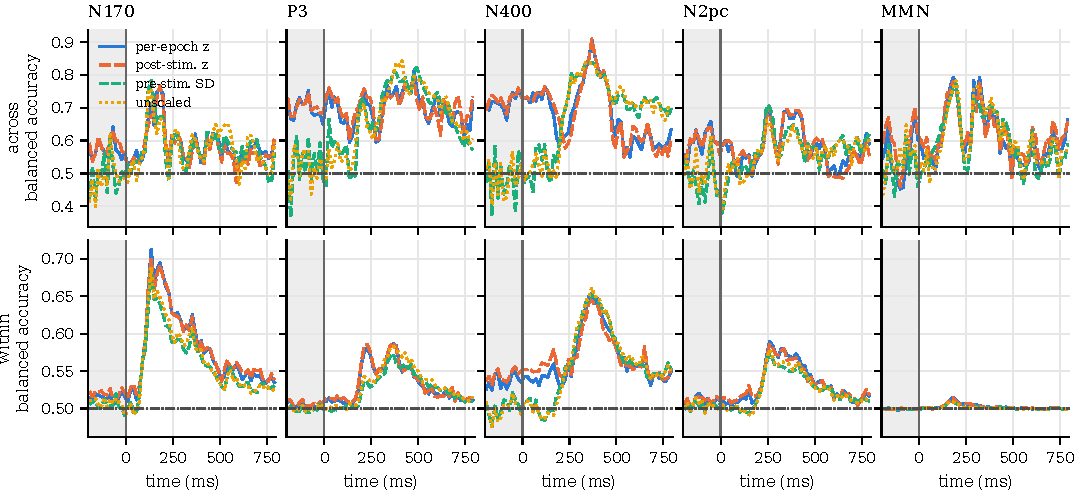
\includegraphics[width=\textwidth]{figures/fig_erpcore.pdf}
\caption{ERP CORE time-resolved decoding of the 28-channel pattern in 15.6~ms bins, chance 0.5 (dash-dot), pre-stimulus interval shaded. Top: across participants (trials scaled, then averaged). Bottom: within participants (single trials, mean over participants). Under per-epoch and post-stimulus z-scoring the curves rise above chance before onset.}
\label{fig:erpcore}
\end{figure*}

\subsection{The Averaging Law}
Fig.~\ref{fig:averaging} tests \eqref{eq:pred} within participants, with the prediction for every $k>1$ computed from the observed single-trial accuracy alone. For N170, N400, and N2pc the predicted curve runs inside the 95\% interval of the observed curve at every $k$. N400 rises from 0.538 at $k=1$ to 0.595 at $k=8$ against a prediction of 0.607, and N2pc from 0.506 to 0.530 at $k=16$. MMN starts at 0.500, where $\Phi^{-1}(\BA(1))=0$, and the law predicts no growth. The observed curve stays between 0.498 and 0.503 for all $k$, an internal control whose brief, sign-changing difference barely moves the epoch mean. P3 rises faster than predicted, reaching 0.538 at $k=4$ against 0.509. Its single-trial estimate, 0.504, lies where $\Phi^{-1}$ amplifies sampling error, and its rare condition supports averages up to $k=4$. Under pre-stimulus scaling every paradigm stays within 0.489 to 0.507 for every $k$.

\begin{figure*}[t]
\centering
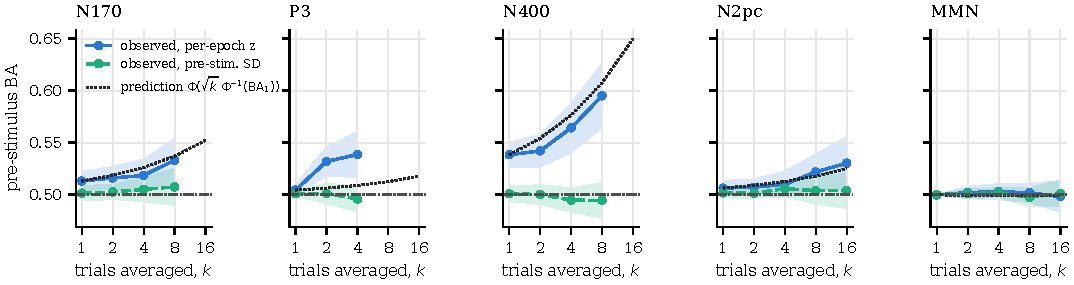
\includegraphics[width=\textwidth]{figures/fig_averaging.pdf}
\caption{The averaging law on ERP CORE, within participants. Pre-stimulus decoding of pseudo-trials averaged over $k$ trials, mean and 95\% interval over participants. Dotted: the prediction $\Phi(\sqrt{k}\,\Phi^{-1}(\BA_1))$ computed from the observed $k=1$ value alone. P3 stops at $k=4$ because its rare condition has too few trials per fold.}
\label{fig:averaging}
\end{figure*}

\subsection{Prevalence of Epoch-Own Scaling}
The audit protocol was committed before any item was inspected \cite{repo_sequel}. Among ten widely used EEG decoding codebases, three scale each sample by its own statistics in their default or reported pipelines: TorchEEG \cite{zhang2024torcheeg} (\texttt{MeanStdNormalize} without supplied statistics), BENDR through the DN3 \texttt{MappingDeep1010} transform (per-trial min-max scaling into $[-1,1]$), and BIOT (division by each sample's 95th amplitude percentile, a scale-only form). Two codebases use training or causal running statistics (braindecode \cite{schirrmeister2017deep}, EEG Conformer \cite{song2023conformer}), four apply a fixed constant (EEGNet reference code \cite{lawhern2018eegnet}, LaBraM \cite{jiang2024labram}, CBraMod \cite{wang2025cbramod}, EEGPT \cite{wang2024eegpt}), and one applies no amplitude scaling (MOABB pipelines \cite{jayaram2018moabb}).

In a fixed-rule sample of the 40 most recent arXiv papers reporting supervised EEG decoding, 28 (70\%) contain no sentence that determines the input scaling. Of the other 12, four scale each window or trial by its own statistics, three use training or participant-wide statistics, one the pre-stimulus interval, three a fixed constant, and one none. Every item and its deciding line are listed in the repository.

\subsection{Location and Scale Routes}
Table~\ref{tab:routes} separates the two propositions on SHAPE and measures the audited transforms. Epoch centering alone reproduces the first-order leak (pre-stimulus mean 0.569 [0.536, 0.602]) and leaves the pre-stimulus log-SD at 0.332, its unscaled value. Scale-only normalization does the reverse. The pre-stimulus mean stays at 0.349, inside its permutation null ($p=0.25$), and the pre-stimulus log-SD rises to 0.450 [0.417, 0.483] ($p=0.005$, the floor of 200 permutations), $+0.118$ [$+0.074$, $+0.163$] above unscaled input. Division by the 95th amplitude percentile behaves as a scale statistic (0.336 and 0.449), and per-epoch min-max scaling leaks through both routes (0.488 and 0.403). The onset-truncated reservoir, a nonlinear encoder, reads both routes: 0.461 under centering, 0.365 under scale-only normalization ($+0.072$ [$+0.021$, $+0.125$] above unscaled input), and 0.355 under percentile scaling ($+0.063$ [$+0.013$, $+0.112$]). The general identity \eqref{eq:general} holds on every epoch to within $1.6\times10^{-15}$ on SHAPE and $1.8\times10^{-15}$ on ERP CORE.

On ERP CORE the location route replicates. Epoch centering alone gives 0.688 for P3 and 0.762 for N400 on a four-bin pre-stimulus pattern ($p=0.002$ each with 500 permutations, Holm-adjusted 0.010 over the five paradigms), and scale-only and percentile scaling leave that pattern inside its null in all five paradigms. The scale route is weaker for single trials, whose $\hat\sigma$ is dominated by background activity. The pre-stimulus log-SD under scale-only normalization reaches 0.620 for N400 ($p=0.008$, adjusted 0.040) and 0.585 for P3 ($p=0.046$, adjusted 0.18), and stays inside its null for N170, N2pc, and MMN.

\begin{table*}[t]
\centering
\caption{SHAPE: the two routes of Propositions~\ref{prop:identity} and~\ref{prop:scale}. Balanced accuracy (participant-bootstrap 95\% CI) of pre-stimulus features under scalings that take a location statistic, a scale statistic, or both from the whole epoch. Three classes, chance 0.333, 211 participants.}
\label{tab:routes}
\begin{tabular}{lcccccc}
\toprule
 & \multicolumn{2}{c}{Statistic from whole epoch} & & & \\
Scaling & location & scale & Pre-stimulus mean & Pre-stimulus log-SD & Reservoir, truncated at onset \\
\midrule
None & -- & -- & 0.340 [0.303, 0.378] & 0.332 [0.297, 0.368] & 0.292 [0.258, 0.330] \\
Pre-stimulus SD & -- & -- & 0.346 [0.313, 0.381] & 0.349 [0.314, 0.382] & 0.297 [0.261, 0.333] \\
Epoch centering & mean & -- & 0.569 [0.536, 0.602] & 0.332 [0.297, 0.368] & 0.461 [0.425, 0.498] \\
Epoch SD (scale only) & -- & SD & 0.349 [0.313, 0.385] & 0.450 [0.417, 0.483] & 0.365 [0.329, 0.403] \\
Epoch 95th percentile & -- & $q_{95}$ & 0.336 [0.300, 0.376] & 0.449 [0.412, 0.485] & 0.355 [0.322, 0.390] \\
Epoch min-max & min & range & 0.488 [0.453, 0.526] & 0.403 [0.367, 0.439] & 0.414 [0.379, 0.447] \\
Epoch z-score & mean & SD & 0.542 [0.507, 0.575] & 0.450 [0.417, 0.483] & 0.420 [0.384, 0.457] \\
\bottomrule
\end{tabular}
\end{table*}



\section{Discussion}\label{sec:discussion}

\subsection{What the Scaling Step Measures}
Proposition~\ref{prop:identity} recasts per-epoch z-scoring as a measurement. Applied to a baseline-corrected epoch, it writes the post-stimulus mean amplitude into every sample, and most visibly into the pre-stimulus interval, where it is the whole of the signal's mean. The SHAPE observations follow the identity closely. A decoder fed $-m/\hat\sigma$ and a decoder fed the pre-stimulus mean of the z-scored epoch reach the same accuracy and agree on 95.9\% of their predictions. The time-resolved analysis shows the second consequence of the same step: every bin carries the epoch mean, so the decoding curve becomes flat in time and its late structure is attenuated. Under per-epoch scaling a decoding time course therefore reports the epoch mean at every latency and loses its meaning as a measurement of when information appears \cite{grootswagers2017decoding,king2014temporal}.

\subsection{Regimes of Leakage}
The averaging law organizes the observations across datasets. In single-trial decoding the leaked feature competes with trial noise, and its effect is small in most paradigms, from 0.4 to 3.7 points. In decoding of averaged data the trial noise shrinks as $1/k$, and the leak approaches the discriminability of the post-stimulus mean itself: 7 to 22 points across participants on ERP CORE and 20 points on SHAPE. Participant-level decoding of averaged ERPs is common in clinical and individual-differences work, where it is also the regime least protected by subject-grouped validation, because the leak lives inside each observation. The law also predicts where the leak is weak. When the condition difference is brief or changes sign within the epoch, as in the MMN, its contribution to the epoch mean is small, and the MMN shows no within-participant leak at any $k$. Across participants its z-scored statistic (0.553, $p=0.045$) sits close to its unscaled value (0.537, $p=0.070$), so its pre-stimulus interval is not a clean null region in the first place.

The prevalence audit places these regimes in current practice. Three of ten widely used codebases scale each sample by its own statistics in their default or reported pipelines, and 70\% of a fixed sample of recent decoding papers leave their input scaling unreported, which leaves the reader without the information needed to assess this leak.


\subsection{Re-Evaluation of the BIBM 2026 Reservoir Result}
The BIBM study characterized the ARSPI-Net temporal encoding stage as a perturbation-characterized measurement operator and reported BA 0.487 for its three-class affective decoding \cite{lane2026bibm}. The present analysis reproduces that value and identifies its source. The spike-count window of that study spans $-160$ to $+73$~ms, and its input epochs were z-scored over their full length. Under scaling that uses no post-stimulus sample, the same reservoir, readout, and protocol score 0.294 [0.262, 0.327], and the onset-truncated reservoir confirms that a causal system acquires the condition information before the stimulus arrives. The decodable content of the BIBM representation is therefore the leaked post-stimulus mean. The two propositions of that study, the chance floor of raw retention and the dependence of zero-fill scores on feature centering, are statements about scoring rules and hold for any input. The magnitudes it reported for them were measured on z-scored input and are re-measured under leak-free scaling as part of the program described below. The firing-rate and damage-spreading measurements describe the reservoir's dynamics under its input, while their link to decoding accuracy requires re-measurement with a post-stimulus read-out window and pre-stimulus scaling.

This re-evaluation was made possible by the transparency of the encoder. A fixed reservoir with an explicit read-out window can be truncated at onset, and that single manipulation separated genuine dynamics from leaked information. The same test applies to any temporal model, as the EEGNet analysis shows.

\subsection{A Reporting Rule}
Three practices follow directly from the theory. First, both the subtracted and the dividing statistic should come from data that contain no part of the response: the pre-stimulus interval of the same epoch, statistics fitted on training data and applied unchanged to test data, as EEG Conformer does \cite{song2023conformer}, or a causal running estimate \cite{schirrmeister2017deep}. Dropping the mean subtraction is not sufficient, because the scale route survives it (Table~\ref{tab:routes}). Second, every decoding pipeline should report its accuracy on the pre-stimulus interval alone, using the model itself or a second-order feature as the encoder, since a first-order check passes under scale-only normalization. Under a valid pipeline this accuracy sits inside its permutation null, so the check costs one additional run and detects this leak, the filtering displacements of \cite{vandriel2021highpass}, and any other transformation that moves post-stimulus information backward in time. Third, studies that decode averaged ERPs at the participant level should treat per-epoch scaling as a high-risk choice, because the averaging law places them in the regime where the leak is largest.

\subsection{Consequences for Online Systems}
Whole-epoch statistics are available only after the epoch has ended, so a decoder validated offline under per-epoch scaling has no causal implementation that reproduces its input. For a brain-computer interface or a closed-loop rehabilitation system, the practical consequence concerns timing claims more than headline accuracy. On the full epoch the scaling changes EEGNet accuracy by $+0.023$ [$-0.005$, $+0.052$], while on windows that end at or shortly after onset it accounts for the whole margin above chance. Early-decision and anticipatory decoders, and any estimate of the latency at which a class becomes separable, are therefore the analyses to re-examine, and the pre-stimulus null test is the criterion they should meet before deployment.

\subsection{Scope and Future Directions}
The present work characterizes trial-averaged affective ERPs in one cohort of 211 participants and five stimulus-locked paradigms of a public resource. The theory covers any time-domain location or scale statistic estimated from the epoch itself, and extending the measurements to spectral and connectivity features, to response-locked paradigms with a separately defined null interval, and to the window-level normalization used by EEG foundation models are natural next steps. The averaging law treats $\hat\sigma$ as constant, and a second-order account of the random denominator would sharpen the prediction at small $k$. For the ARSPI-Net program, the measurement operator of \cite{lane2026bibm} can now be re-measured with a post-stimulus read-out window and leak-free scaling, which gives its dynamical characterization a clean input on which to stand.


\section*{Data and Code Availability}
SHAPE data are available from the Laboratory for Clinical Affective Neuroscience at Stony Brook University on request \cite{shape}. ERP CORE is public \cite{kappenman2021erpcore}. All code, the committed predictions, and every aggregate result reported here are public \cite{repo_sequel}. No participant-level data are included in the repository.

\section*{Use of AI-Assisted Tools}
An AI assistant (Claude, Anthropic) was used to write analysis code, run experiments, search and verify the literature, and draft text under the direction of the authors. The authors reviewed every analysis and statement, and take full responsibility for the content.

\bibliographystyle{IEEEtran}
\bibliography{refs}

\end{document}
